\documentclass[11pt]{article}


\setlength{\parindent}{0pt}
\usepackage{xltxtra}
\usepackage{hyperref}
\hypersetup{hidelinks}
\usepackage{url}
\urlstyle{tt}
\usepackage{xcolor}
\definecolor{CVBlue}{RGB}{23,110,191}
\usepackage{calc}
\usepackage{graphicx}
\usepackage{tikz}
\usetikzlibrary{calc}
\usepackage{fontspec}
\usepackage{xeCJK}
\usepackage{enumitem}
\CJKsetecglue{} %% 取消中文与数字之间的间隙


%% 主文档字体设置
\setmainfont[
    Path = fonts/Main/,
    Extension = .otf,
    BoldFont = texgyretermes-bold.otf, % 加粗字体
]{texgyretermes-regular.otf} % 正文字体

% 中文字体设置
\setCJKmainfont[
    Path = fonts/hansans/,
    Extension = .ttf,
    BoldFont = NotoSansSC-Bold.ttf, % 加粗字体
]{NotoSansSC-Regular.otf} % 正文字体


\usepackage{relsize}
\usepackage{xspace}

% 使用 fontawesome（部分图标）
\usepackage{fontawesome} 

% A4纸，上下左右边距
\usepackage[
    a4paper,
    left=1.2cm,
    right=1.2cm,
    top=1.5cm,
    bottom=1cm,
    nohead
]{geometry}

\renewcommand{\baselinestretch}{1.5} % 行间距设为1.5

\usepackage{titlesec}
\usepackage{enumitem}
\setlist{noitemsep} % 取消列表项间的额外间距
%\setlist{nosep} % 取消所有垂直间距
\setlist[itemize]{topsep=0.25em, leftmargin=*}
\setlist[enumerate]{topsep=0.25em, leftmargin=*}

% --- 用于控制【不同项目之间】的垂直距离 ---
\newlength{\interProjectSpacing}
\setlength{\interProjectSpacing}{0.9em} % <--- 在此调整项目之间的距离
\newcommand{\projectsep}{\vspace{\interProjectSpacing}}

% --- 用于控制【项目标题】与下方【项目描述】的距离 ---
\newlength{\intraProjectTitleSep}
\setlength{\intraProjectTitleSep}{0.4em} % <--- 在此调整标题和描述的距离
\newcommand{\titlebreak}{\\[\intraProjectTitleSep]}

% --- 用于控制【项目描述】与下方【要点列表】的距离 ---
\newlength{\intraProjectListTopSep}
\setlength{\intraProjectListTopSep}{0.2em} % <--- 在此调整描述和列表的距离

% =======================================================================


\titleformat{\section}         % 定制 \section 命令 
{\large\bfseries\raggedright} % 将 section 标题设置为大号、粗体且左对齐
{}{0em}                      % 可用于为所有 section 添加前缀（如“章节...”）
{}                           % 可用于在标题前插入代码
[{\color{CVBlue}\titlerule}]  % 在标题后插入一条横线
\titlespacing*{\section}{0cm}{*1.6}{*1.2}



\begin{document}
\pagenumbering{gobble}

%%%% 利用tikz来定位照片
\begin{tikzpicture}[remember picture, overlay] 
    \node[anchor = north east] at ($(current page.north east)+(-2cm,-1.2cm)$) {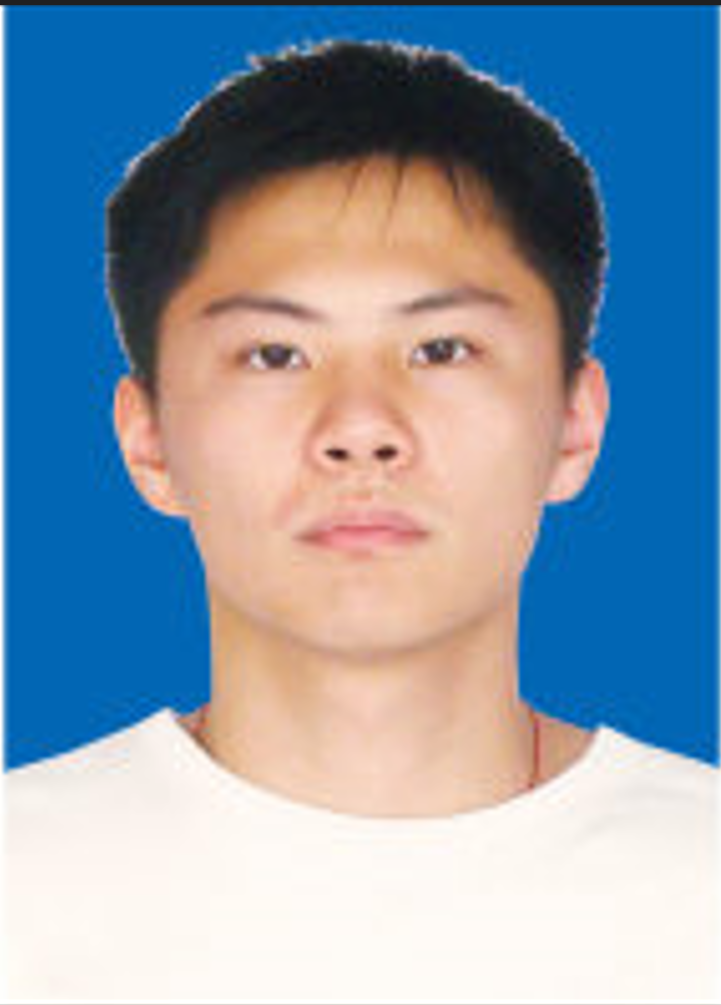
\includegraphics[height=3cm]{avatar.jpg}};
  \end{tikzpicture}%
  %%%% 利用tikz来定位学校Logo，这里只在第一页显示
  \begin{tikzpicture}[remember picture, overlay] 
    \node[anchor = north west] at ($(current page.north west)+(0.5cm,+1.0cm)$) {\includegraphics[height=6cm]{zju.png}};
  \end{tikzpicture}%
\centerline{\LARGE\bfseries{康鑫堡}} 
\vspace{0.2em}
\centerline{\normalsize{\faUser\ 中共党员}}
\vspace{0.2em}
\centerline{\normalsize{\faPhone\ 195-5820-8920 \quad \faEnvelopeO\ xinbao\_kang@zju.edu.cn}} 
    
\section{\makebox[\widthof{\faGraduationCap}][c]{\color{CVBlue}\faGraduationCap}\ 教育背景}    
\textbf{浙江大学电气工程学院} \quad \textbf{电子信息工程专业} \hfill 2023.09 -- 2027.06\\[0.1em] % 同行并列显示
\begin{itemize}[nosep, topsep=-0.2em] % 缩减空白
    \item \textbf{学业表现}：综合排名 19/74，综合绩点 4.81，荣获浙江大学一等奖学金、国家励志奖学金、浙江大学郭谢碧蓉奖学金（二类）等。
    \item \textbf{相关课程}：电路与电子技术II（93分）、信号分析与处理（92分）、通信原理（90分）、信息论与编码（90分）、电力电子技术（89分）、离散数学（89分）等。
\end{itemize}

\section{\makebox[\widthof{\faUsers}][c]{\color{CVBlue}\faUsers}\ 学术与项目经历}

% --- 中国高校智能机器人创意大赛 ---
\textbf{中国高校智能机器人创意大赛（仿人机器人格斗 A 赛道 ｜ 统一部件组）} \hfill 2025 -- 2026 学年 \\
\textbf{项目角色}：第一负责人 \hfill \textbf{获得奖项}：国家一等奖 \\
主导基于高阶有限状态机（FSM）的自主任务调度开发，设计巡线 PD 控制器抑制偏航，并优化 IMU 接收队列彻底消除动作延迟累积；将 YOLOv5m 目标检测部署于 RK3588S 边缘端，利用 OpenCV 黑边填充预处理实现 AprilTag 与武器稳定识别（达 95\%）；利用逆向分析工具反编译加密固件（.BIN），破除底层 0.3 的运动速度限制。

\projectsep

% --- 高校电气电子工程创新大赛 ---
\textbf{高校电气电子工程创新大赛（企业赛道）} \hfill 2025 -- 2026 学年 \\
\textbf{项目角色}：核心研发成员 \hfill \textbf{获得奖项}：浙江省二等奖 \\
负责核心控制算法研发。针对企业赛道高功率密度指标要求，参与研发了高效率同步升降压（Buck-Boost）DC-DC 变换器；基于 STM32G4 单片机在中断中实现了双环 PI（电压外环、电流内环）数字闭环控制算法，主导了双层 PCB 电磁抗干扰设计，变换器实测满载效率达 96.5\%。

\projectsep

% --- ZPEC 论文 ---
\textbf{2026 IEEE 浙江电力电子国际会议（ZPEC 2026）录用学术论文（4/6）} \hfill 2026.08 \\
于第二届浙江电力电子国际会议录用学术论文 1 篇，研究局部阴影条件（PSC）下的光伏全局最大功率点快速无振荡跟踪技术。负责其中高频双向 DAB 变换器建模仿真，利用分段驱动电流优化有源门极驱动（AGD）开关瞬态 $dv/dt$ 控制，抑制高频共模噪声并宽展零电压开关（ZVS）软开关范围。\\
\textit{论文引用：D. Chen, ..., ..., \textbf{X. Kang}, ..., Y. Yang, ``A Photovoltaic GMPPT Method Based on Region Segmentation Principle and Shallow Decision Tree,'' in Proc. ZPEC, 2026. (Accepted)}


\section{\makebox[\widthof{\faUsers}][c]{\color{CVBlue}\faUsers}\ 学生工作}

\textbf{班级与团支部管理} \hfill 2023.09 -- 至今 \\
\textbf{电信 2302 班 班长}：统筹日常班委会建设与班级事务，因工作成果优异，获评校级、园级“优秀团干部”； \\
\textbf{工科试验班 2323 团支部书记}：组织开展支部日常管理与思想作风建设，引导支部青年思想凝聚，获评园级“优秀团干部”。

\projectsep

\textbf{学长组建设} \hfill 2024.09 -- 2025.06 \\
\textbf{24 级学长组 组长}：主导新生学业生涯规划与破冰引导。方案获评“蓝田学长组优秀破冰方案”，个人获“校级优秀学长”及“园级优秀学长组”荣誉。

\projectsep

\textbf{学生组织经历} \hfill 2024.09 -- 2025.06 \\
在校内多个优秀团队中任职。在\textbf{图书馆学生助管中心（系统研发部）}负责服务网站日常运维、安全状态监控与更新；在\textbf{机械学院考拉工作室（运营部）}主导自媒体平台运营规划与大型品牌宣发；在\textbf{“求是潮”视频团队}参与多项校级宣传微视频的选题、拍摄与后期制作。


\section{\makebox[\widthof{\faInfo}][c]{\color{CVBlue}\faInfo}\ 社会实践与志愿服务}
\textbf{志愿服务（五星志愿者 ｜ 现场服务组长）} \hfill 累计服务近 350 小时 \\
担任 2024 年“缘定浙大”大型校友活动组长，统筹近百名志愿者的排班调度、物资分配与现场突发应急处理。

\projectsep

\textbf{社会实践与回访宣讲} \hfill 2024.01 -- 2024.07 \\
赴基层农户开展乡村调研并参与社会调查报告撰写；回访义乌二中主讲浙大宣讲会，宣讲成果评比最终斩获校级一等奖。


\section{\makebox[\widthof{\faGraduationCap}][c]{\color{CVBlue}\faList}\ 荣誉奖项}
\begin{itemize}[nosep]
    \item \textbf{国家励志奖学金} \hfill \textbf{浙江大学一等奖学金}
    \item \textbf{浙江大学郭谢碧蓉奖学金（二类）} \hfill \textbf{浙江大学“优秀学生”荣誉称号}
    \item \textbf{浙江大学社会工作标兵、学业优秀标兵、公益服务标兵、对外交流标兵}
    \item \textbf{浙江大学校级优秀学长} \hfill \textbf{浙江大学校级优秀团干部}
    \item \textbf{电气工程学院优秀团干部} \hfill \textbf{浙江大学五星志愿者（服务近 350 小时）}
\end{itemize}
    

\section{\makebox[\widthof{\faCogs}][c]{\color{CVBlue}\faCogs}\ 专业技能}
\begin{itemize}[nosep]
    \item \textbf{控制工程与电力电子}：精通基于 RK3588S、STM32 平台的机电系统与电力电子系统开发。熟练掌握高阶有限状态机（FSM）任务流调度与电机 PD 闭环控制算法；精通高频双向 DC-DC 变换器设计，掌握基于 Simulink 的光伏并网系统建模仿真及 GMPPT 算法。
    \item \textbf{逆向工程与底层开发}：具备实用的二进制软件逆向与反编译实战经验，熟悉固件编译产物（.BIN 二进制文件）的静态反汇编分析与底层调试技术，具备定位芯片级限制、执行二进制代码打补丁（Binary Patching）的底层开发与 IMU 串口数据流优化能力。
    \item \textbf{图像视觉与综合素质}：熟练掌握 YOLOv5m 在嵌入式边缘端的轻量化部署与实时推理，熟悉 OpenCV 图像黑边填充防拉伸预处理与 AprilTag 目标识别；英语水平良好（通过 CET-4, CET-6），熟练使用 LaTeX 进行英文学术论文排版。
\end{itemize}
\end{document}